
\documentclass{beamer}
\usepackage{HECbeamer}
% \usepackage{pgfpages}
% \pgfpagesuselayout{4 on 1}[letterpaper, landscape, border shrink=5mm]
\title[\color{white}{MATH 60604A \S~4e - Contingency tables}]{\texorpdfstring{MATH 60604A \\Statistical modelling \\ \S~4e - Contingency tables}{MATH 60604A \\Statistical modelling \\ \S~4e - Contingency tables}}
\author{Léo Belzile}
\institute{HEC Montréal\\
Department of Decision Sciences}
\date{} 

\begin{document}
\frame{\titlepage}
\begin{frame}[fragile]
 \frametitle{Two-way contingency tables}
 The most common format for aggregated count data with categorical predictors is \textbf{contingency tables}, in which each cell is a count for a given combination of levels of the categorical variables.
 
 
 Consider $\mathrm{X}_1$ and $\mathrm{X}_2$ two categorical variables with $J$ and $K$ levels and the associated contingency table. 
 \begin{center}
  \begin{tabular}{c|cccc}
   &$\mathrm{X}_2=1$ & $\mathrm{X}_2=2$ & $\cdots$ & $\mathrm{X}_2=K$\\\specialrule{\cmidrulewidth}{0pt}{0pt}
   $\mathrm{X}_1=1$ & $Y_{11}$ & $Y_{12}$ & $\cdots$ & $Y_{1K}$ \\
   $\mathrm{X}_1=2$ & $Y_{21}$ & $Y_{22}$ & $\cdots$ & $Y_{2K}$ \\
  $\vdots$  & $\vdots$ & $\ddots$  & $\ddots$ &  $\vdots$ \\
  $\mathrm{X}_1=J$ & $Y_{J1}$ & $Y_{J2}$ & $\cdots$ & $Y_{JK}$
 \end{tabular}
\end{center}

\end{frame}
\begin{frame}
\frametitle{Testing independence in contingency tables}
\bi \item We consider two competing Poisson models: under $\Hy_0$, a model with the two categorical variables, but \textbf{no interaction}. For $(j= 1, \ldots, J; k=1, \ldots, K)$, the mean number in cell $(j,k)$ is
 \begin{align*}
  \mu_{jk} = \exp\left(\beta_0 + \alpha_j \I{\mathrm{X}_{1}=j} + \gamma_k \I{\mathrm{X}_{2}=k}\right),
 \end{align*}
with $\alpha_1=0$ and $\gamma_1=0$ for identifiability. 
\item 
The alternative model is the saturated model (including an additional interaction between  $\mathrm{X}_1$ and $\mathrm{X}_2$).   The null hypothesis of  \alert{independence} is simply a test that the additional parameters associated to the interaction are equal to zero.
\ei 
\end{frame}
\begin{frame}
 \frametitle{Main effects and saturated models for two-way contingency tables}
 \bi \item Under $\Hy_0$, the model includes only $\mathrm{X}_1$ and $\mathrm{X}_2$ (main effects). 
  \bi 
  \item One can show that the fitted values of the null model are the product of the sample proportion in each line/column. 
  \item We denote the fitted values for cell $(j,k)$ is denoted $\hat{\mu}_{jk}$.
  \ei
  \item The saturated model, under the alternative $\Hy_1$, includes additional parameters for the interaction.
    \bi \item the saturated model has $n=JK$ parameters and the fitted values are simply $Y_{jk}$.
\ei 
\ei 
\end{frame}
\begin{frame}
\frametitle{Statistics for the test of independence in contingency tables}
\bi
 \item The likelihood ratio test statistic is the deviance, 
  \begin{align*}
   D= 2 \sum_{j=1}^J \sum_{k=1}^K Y_{jk}\ln \pfrac{Y_{jk}}{\hat{\mu}_{jk}},
  \end{align*}
which follows $\chi^2_{(J-1)(K-1)}$ under the null hypothesis of independence.
\item Alternatively, we can use the score test statistic (with the same null distribution), 
\begin{align*}
 X^2 = \sum_{j=1}^J \sum_{k=1}^K \frac{(Y_{jk}-\hat{\mu}_{jk})^2}{\hat{\mu}_{jk}}.
\end{align*}
  \ei 
\end{frame}
\begin{frame}[fragile]
 \frametitle{Political affiliation in USA}
 We consider the two by three contingency table of political affiliation by party in the US as a function of gender in 2000.
 \begin{center}
 \begin{tabular}{llllc}
 \toprule 
  & \multicolumn{3}{c}{Party Identification} & \\
  \cmidrule(r){2-4}
  Gender & Democrat & Independent & Republican & Total\\
  Females & $762$ & $327$ & $468$ & $1557$ \\
   & ($703.7$) & ($319.6$) & ($533.7$) & \\
   Males & $484$ & $239$ & $477$ & $1200$ \\
    & ($542.3)$ & $(246.4)$ & $(411.3)$ & \\
    Total & $1246$ & $566$ & $945$ &$2757$\\
    \bottomrule 
    \end{tabular}
    \end{center}
    The number in parenthesis represent the fitted values from the additive Poisson model without interaction (main effects).

     
  {   \footnotesize
 Data reproduced from Table 2.5, Agresti (2007), \textsl{An Introduction to
Categorical Data Analysis}, Wiley.


}
\end{frame}
\begin{frame}
 \frametitle{Result of the independence test for political affiliation}
   \bi \item     
By fitting the model without interaction, we get the $X^2$ and the likelihood ratio statistic in the output ($30.07$ and $30.02$, respectively).
\item Both should behave as $\chi^2_2$ variables if gender was independent of political affiliation. 
\item The $p$-values are smaller than $10^{-4}$ and we conclude against independence, meaning gender has an effect on political affiliation.
\ei
\begin{center}
 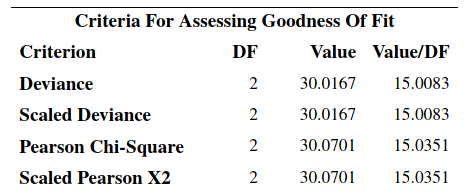
\includegraphics[width = 0.6\linewidth]{img/c4/slides8-e1}
\end{center}
\end{frame}



\end{document}
